\textbf{B.5: 3D Taret Modeli}
\label{SekizinciBolum}

Taretin baskısı 3D yazıcılar vasıtasıyla PLA+  Filament kullanılarak yapıldı. Kendi oluşturmuş olduğum 3D modelleri ile Github üzerindeki üyerlerin modellerini mix ederek aşağıdaki modelleri elde etmiş oldum. 3D modeli oluşturmak için Blender programını kullandım. Taretin 3D modelleri Şekil 9’da gösterilmiştir. KAYNAK [1]

\begin{figure}[H]
	\centering
	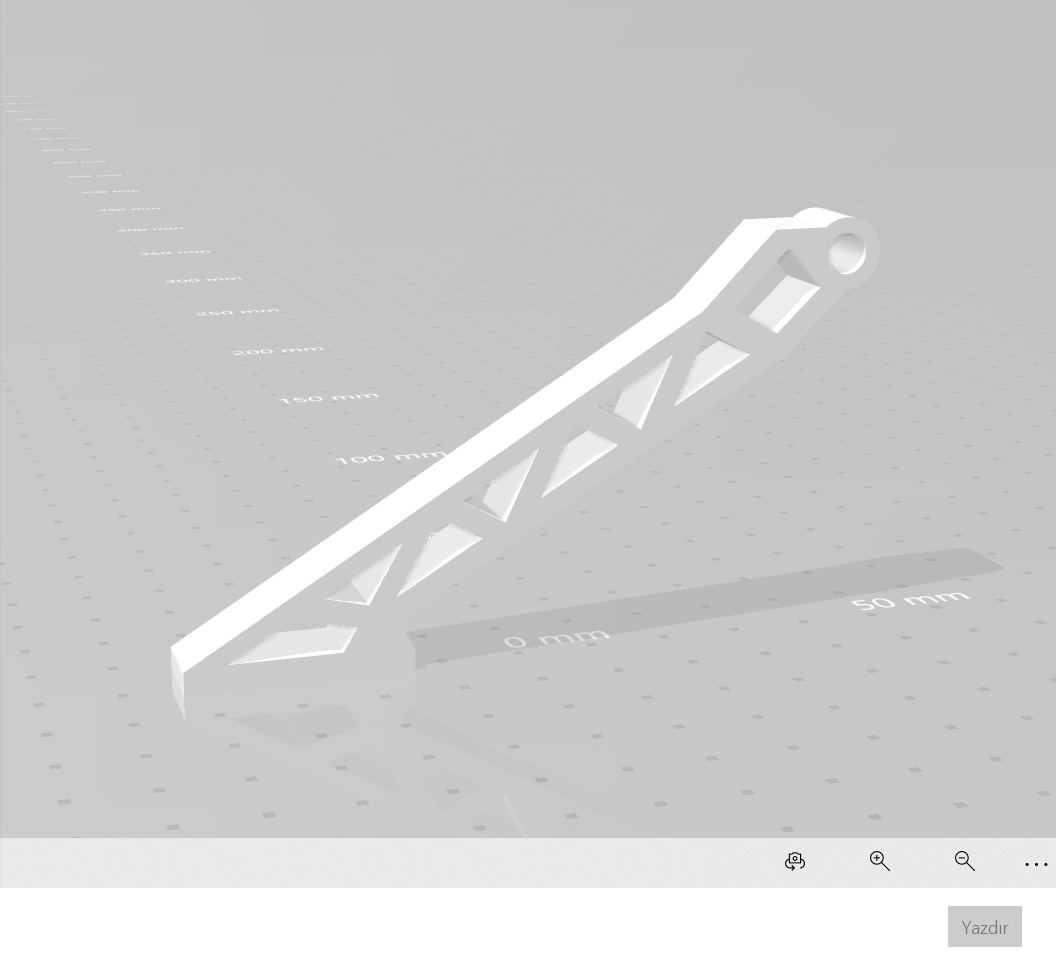
\includegraphics[width=50mm]{grafik/3D_Bacak.png}
    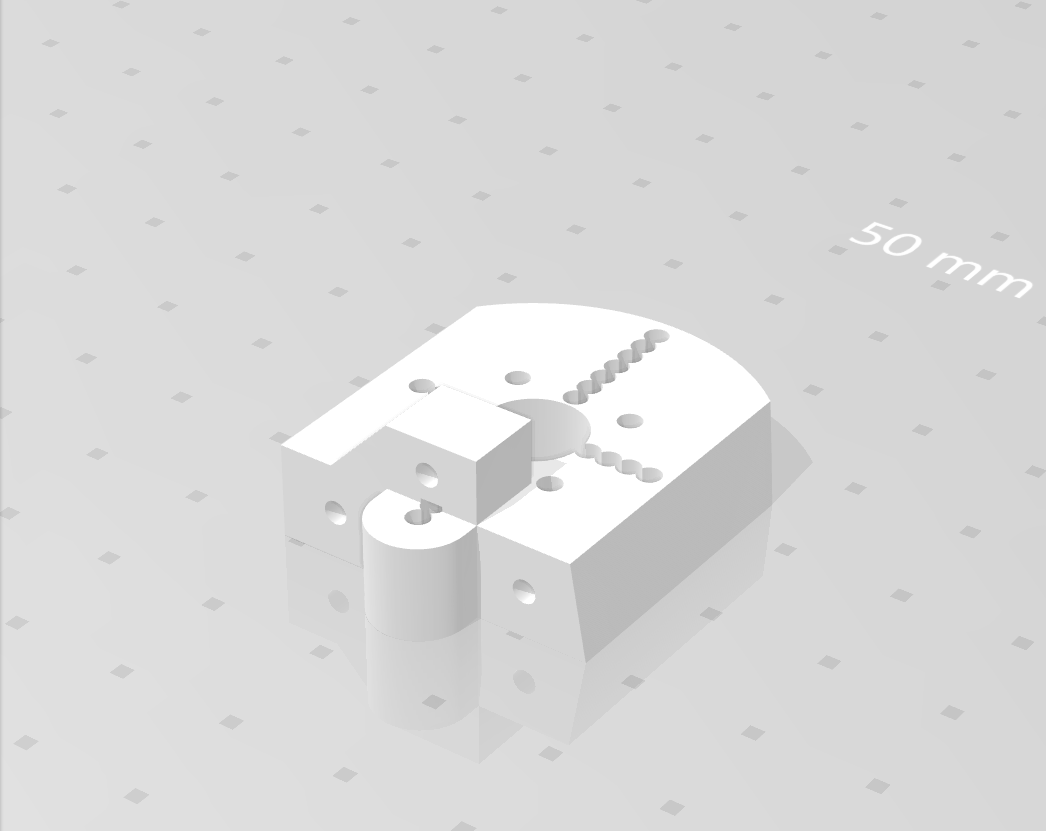
\includegraphics[width=50mm]{grafik/3D_EgilimAltDestegi.png}
    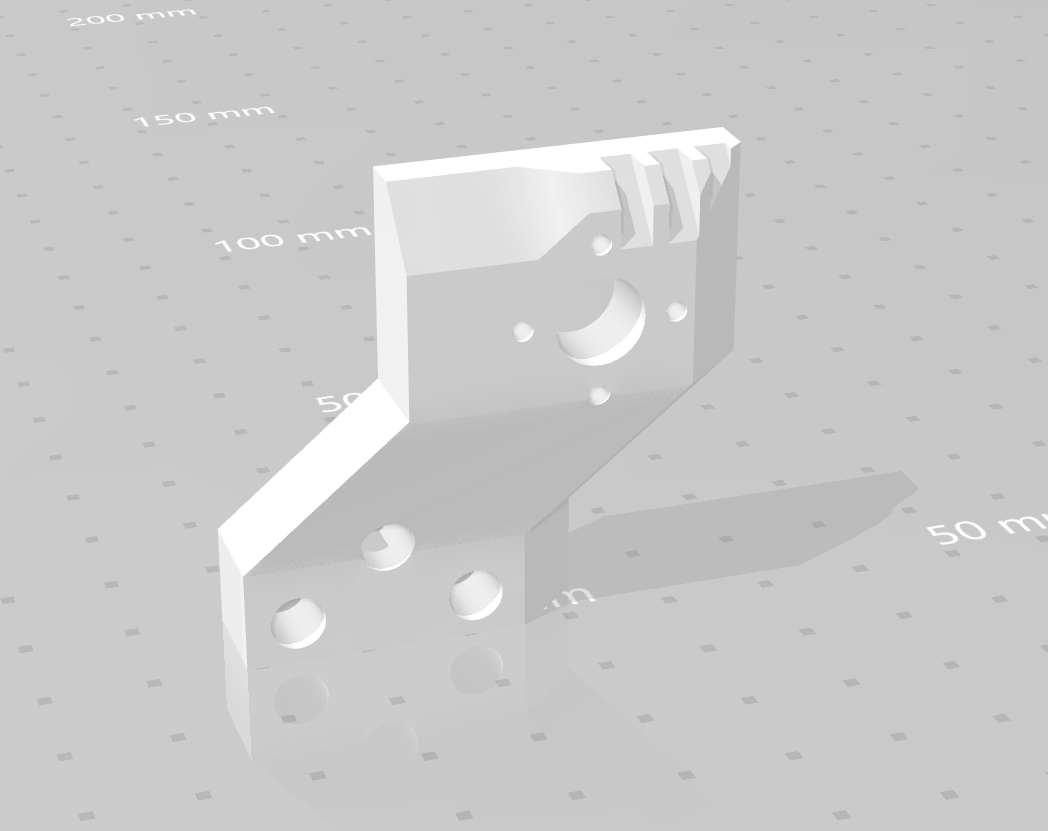
\includegraphics[width=50mm]{grafik/3D_EgilimUstDestegi.png}
    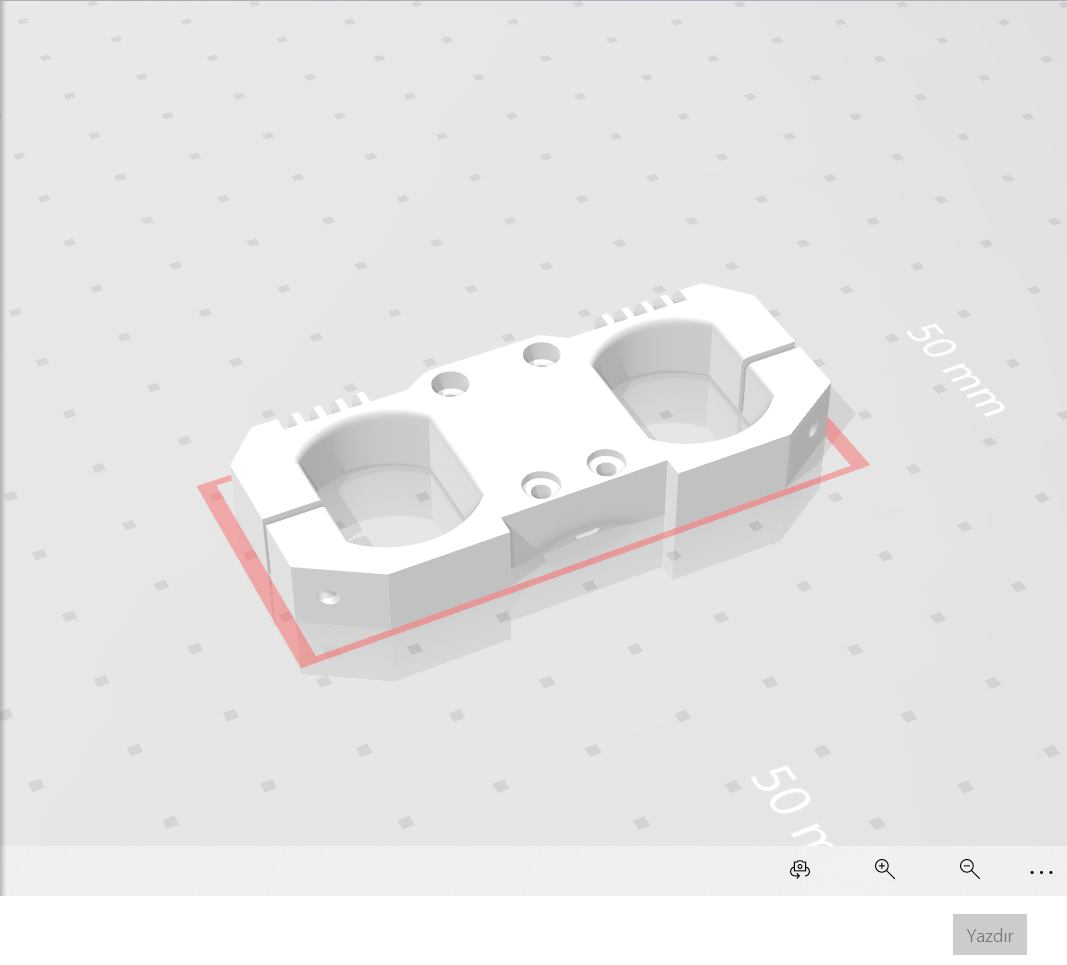
\includegraphics[width=50mm]{grafik/3D_MotorDestek.png}
    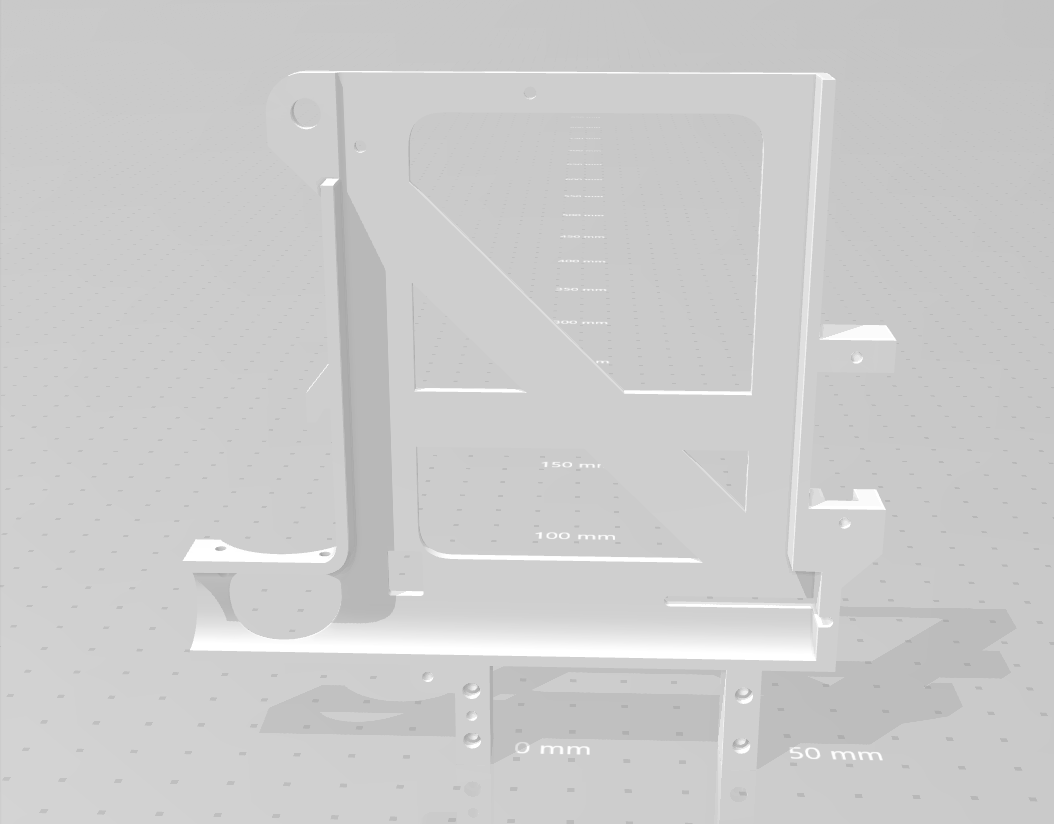
\includegraphics[width=50mm]{grafik/3D_NamluPlatformu.png}
    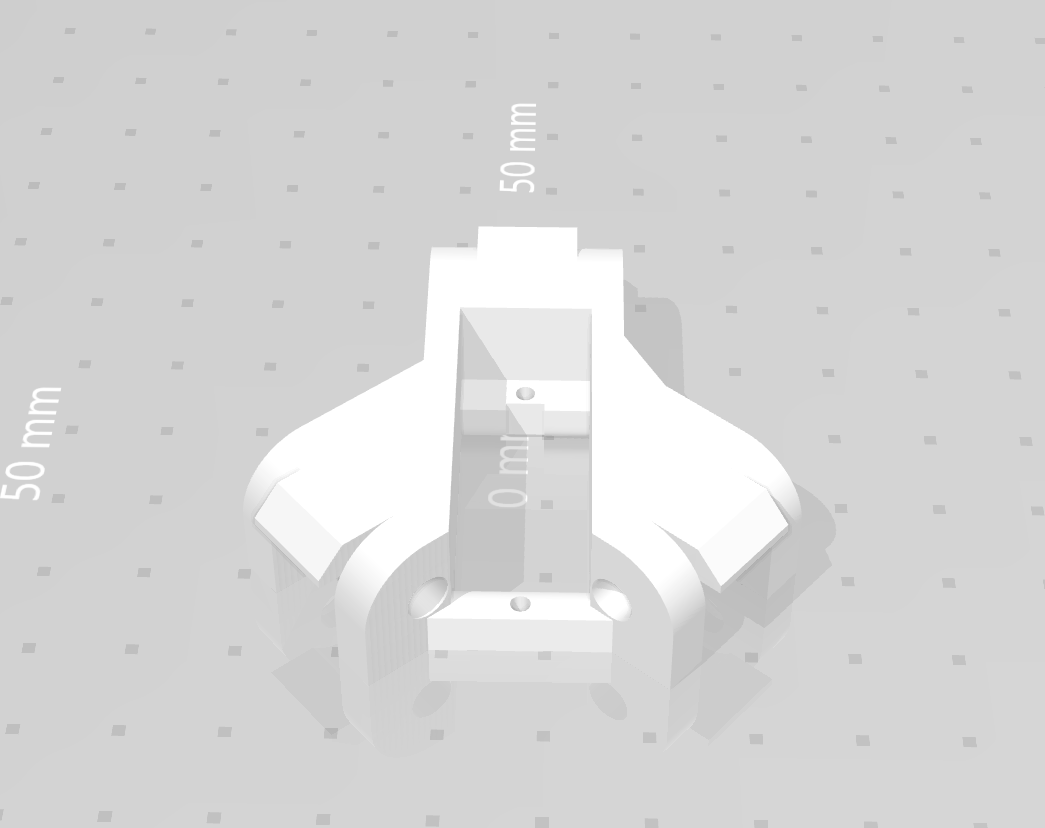
\includegraphics[width=50mm]{grafik/3D_Temel.png}
    
    \caption{Taret 3D Model Örnekleri}
    \label{fig:Taret1,2,3,4,5,6DM}
\end{figure}

\clearpage